\noindent
This section argues that it is both practical and useful
to use AI to help SLRs since
as argued in  the introduction,  the space of SE papers is not large. Hence, AI tools can efficiently 
explore this space. Also:
\bi
\item
As argued in \tion{useful}, our initial prototypes show much promise in AI-enhanced SLR tools.
\item
As argued in \tion{canai}, AI-augmented SLR tools can address the requirements listed in
\tion{results}.
\ei
Further, if {\IT} caches prior results then it is highly likely that subsequent queries can reuse, at least in part,
older results. 
\vspace{8pt}

% \begin{wraptable}{r}{2in}
% \small
% \begin{tabular}{|p{1.8in}|}\hline
% \bii
% \item
% Conferences: 
% MDLS, RE, ESEM, SSBSE, MSR, WCRE, ICPC, ICSM (ICSME), CSMR, ICSE, SANER, FSE, ASE, SCAm, GPCE, FASE.
% \item
% Journals: SOSYM, IEEE Software, REJ, SESE, SEM, SQJ, IST, ISSE, IJSEKE, NOTES, JSS, SOE, STVR, ASEJ, TSE, TOSEM
% \eii\\\hline
% \end{tabular}
% \caption{Some SE venus to use in SLRs.}\label{tbl:where}
% \end{wraptable}
% Before arguing for  three points,
% it  
% should be stressed that:
% \bi
% \item
% As seen in the middle column of \tbl{overview},
% many parts of the SLR process are best done using manual methods or automatic methods
% that make no use of AI (for more on this point, see next section).
% \item
% Also, an  important part of our methods is that humans and AI work together in partnership
% to achieve some goal. So when we say  ``AI methods'', we might more accurately say  ``AI  working
% in partnership with human beings.''
% \ei
% \begin{table}[!t]

\caption{The top 7 terms in the 10 major SE topics
as found by AI text mining tools from 35,391 papers published at
major  conferences (MDLS, RE, ESEM, SSBSE, MSR, WCRE, ICPC, ICSM (ICSME), CSMR, ICSE, SANER, FSE, ASE, SCAm, GPCE, FASE) and major journals
(SOSYM, IEEE Software, REJ, SESE, SEM, SQJ, IST, ISSE, IJSEKE, NOTES, JSS, SOE, STVR, ASEJ, TSE, TOSEM)
in the period 1992 to 2016.
This table show just the top  seven terms in each cluster since there is an exponential drop in their frequency and ``knee'' of that curve occurs at terms=7. 
Topics are ordered top-to-bottom, most-to-least frequent. Also, terms within topics are ordered left-to-right most-to-least frequent. Topics are 
named using the most frequent terms. These topics cover 95\% of the papers studies by Mathew, Menzies et al.~\cite{Mathew_2018,mathewSoft18}.
}
\label{tbl:11topics}
{\footnotesize
  \begin{center}
\begin{tabular}{r@{~=~}l}\hline
  Source Code & code, source, information, tool, program, developers, patterns \\
  \textcolor{black}{Software process} & requirements, design, systems, architecture, analysis, process, development \\
  Modeling & model, language, specification, systems, techniques, object, uml \\
  Program Analysis & program, analysis, dynamic, execution, code, java, static \\
  Metrics & metrics, data, quality, effort, prediction, defect, analysis \\
  Developer & developer, project, bug, work, open, team, tools \\
  Applications & applications, web, systems,  component,  services, distributed, user \\
  Testing & test, testing, cases, fault, techniques, coverage, generation \\
  Performance & performance, time, data, algorithm, systems,   problem, network, distributed \\
  Architecture & architecture, component, systems, design, product,  reuse, evolution  
   \\\hline

\end{tabular}
\end{center}}
\end{table}
% %\begin{figure*}[!t]
\centering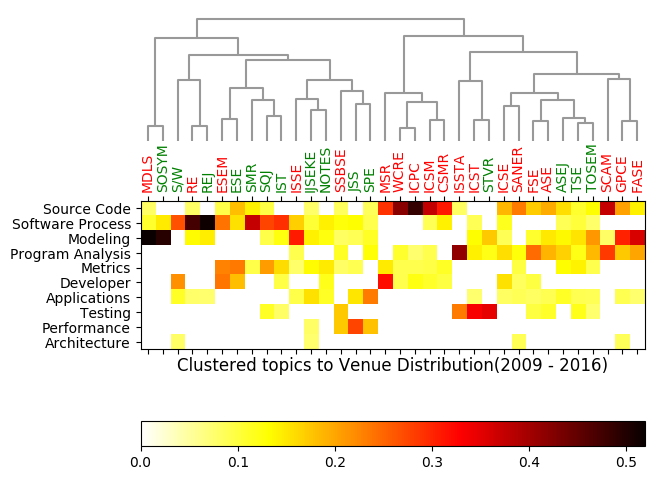
\includegraphics[scale=0.7]{png_heatmap_09_16_dend.png}
\caption{Hierarchical clustering heatmap of 35,000+ 
papers and SE Venues over the last 25 years.
Along the top,  \textcolor{ao(english)}{{\bf green}} denotes
journals and   \textcolor{red}{{\bf red}} denotes  conferences.
Along the left side, the black words are the  topics of \tbl{11topics}. 
Topics are sorted top-to-bottom, most-to-least frequent.
Each cell in the heatmap depicts the 
frequency of a topic in a particular
venue.  The tree diagrams above the venues 
show the results of a bottom up clustering of the venues with respect to the topics. In those clusters, venues are in similar
sub-trees if they have similar pattern of topic frequencies. The venues presented in this figure were selected after much interaction with the international community.
Initially, we started with Google Scholar's list of top venues. 
Next, some 
feedback from reviews of a conference  paper~\cite{Mathew2017}  
made us look more broadly at more conferences and  SE journals.
To that list, using our domain knowledge, we added
venues that we knew were associated with senior researchers in the field;
e.g. the ESEM and SSBSE conferences. 
}
\label{fig:div_heat}
\end{figure*}
 

% \subsection{The Space of SE papers is not Large}\label{tion:unlarge}

\subsection{Useful Initial  Results}\label{tion:useful}

\begin{wrapfigure}{r}{2in}
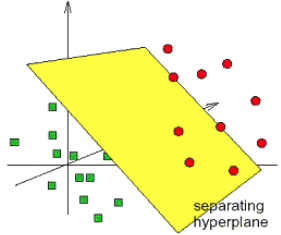
\includegraphics[width=1.5in]{figure_svm.png}
\caption{A support vector machine learns
a  hyperspace boundary between relevant and irrelevant documents (shown here in green and red, respectively).}\label{fig:svm}
\end{wrapfigure}
Our recent prototypes with AI text mining to support SLRs
offers an example of the kinds of results that can be obtained with 
these AI tools.
FASTREAD~\cite{Yu2019,Yu2018} is an {\em active learning} tool that helps
humans find relevant papers, faster.
Active learners like FASTREAD suggest what papers are most/least informative
to read next.   The experience in other domains is that  such  active learning can significantly
reduce the effort required to achieve high
recall~\cite{Cormack2017Navigating,Cormack2016Engineering,cormack2014evaluation,wallace2010semi,wallace2010active,wallace2011should,wallace2013active,Yu2018}. 



To understand active learning, consider the decision plane between the relevant    and   irrelevant
documents 
 of \fig{svm}.
Suppose we want to find more relevant documents and we had access to the  \fig{svm} model. One tactic for quickly finding those relevant documents would be to inspect as-yet-unread documents that fall into the red region of this figure, as far as possible from the green ones (this tactic is called {\em certainty sampling}). Another tactic would be to verify the position of the boundary; i.e. inspect unclassified files that are closest to the boundary (this tactic is called {\em uncertainty sampling}).  Zhe, Menzies et al.~\cite{Yu2018}  found that inter-levering these two tactics was a useful approach (see~\cite{Yu2019,Yu2018} for details).
Compared to manual methods, FASTREAD lets researchers find 95\% relevant studies after reviewing an order of magnitude fewer papers. Compared to other state-of-the-art automatic methods, FASTREAD reviews 20-50\% fewer studies while finding same number of relevant primary studies in a systematic literature review.
\fig{Core} compares FASTREAD against state-of-the-art text mining methods
reported in in domains such as medicine~\cite{wallace2010active,miwa2014reducing}
and legal text mining reasoning~\cite{cormack2014evaluation}.
Note that, in \fig{Core}, the data sets used in that evaluation
all come from prominent and recent software engineering SLRs conducted by Hall, Wahono, Radjenovi{\'c}, Kitchenham et al.~\cite{ wahono2015systematic,hall2012systematic,radjenovic2013software,kitchenham2013systematic}. 

\begin{wrapfigure}{r}{3.55in}
    \centering
    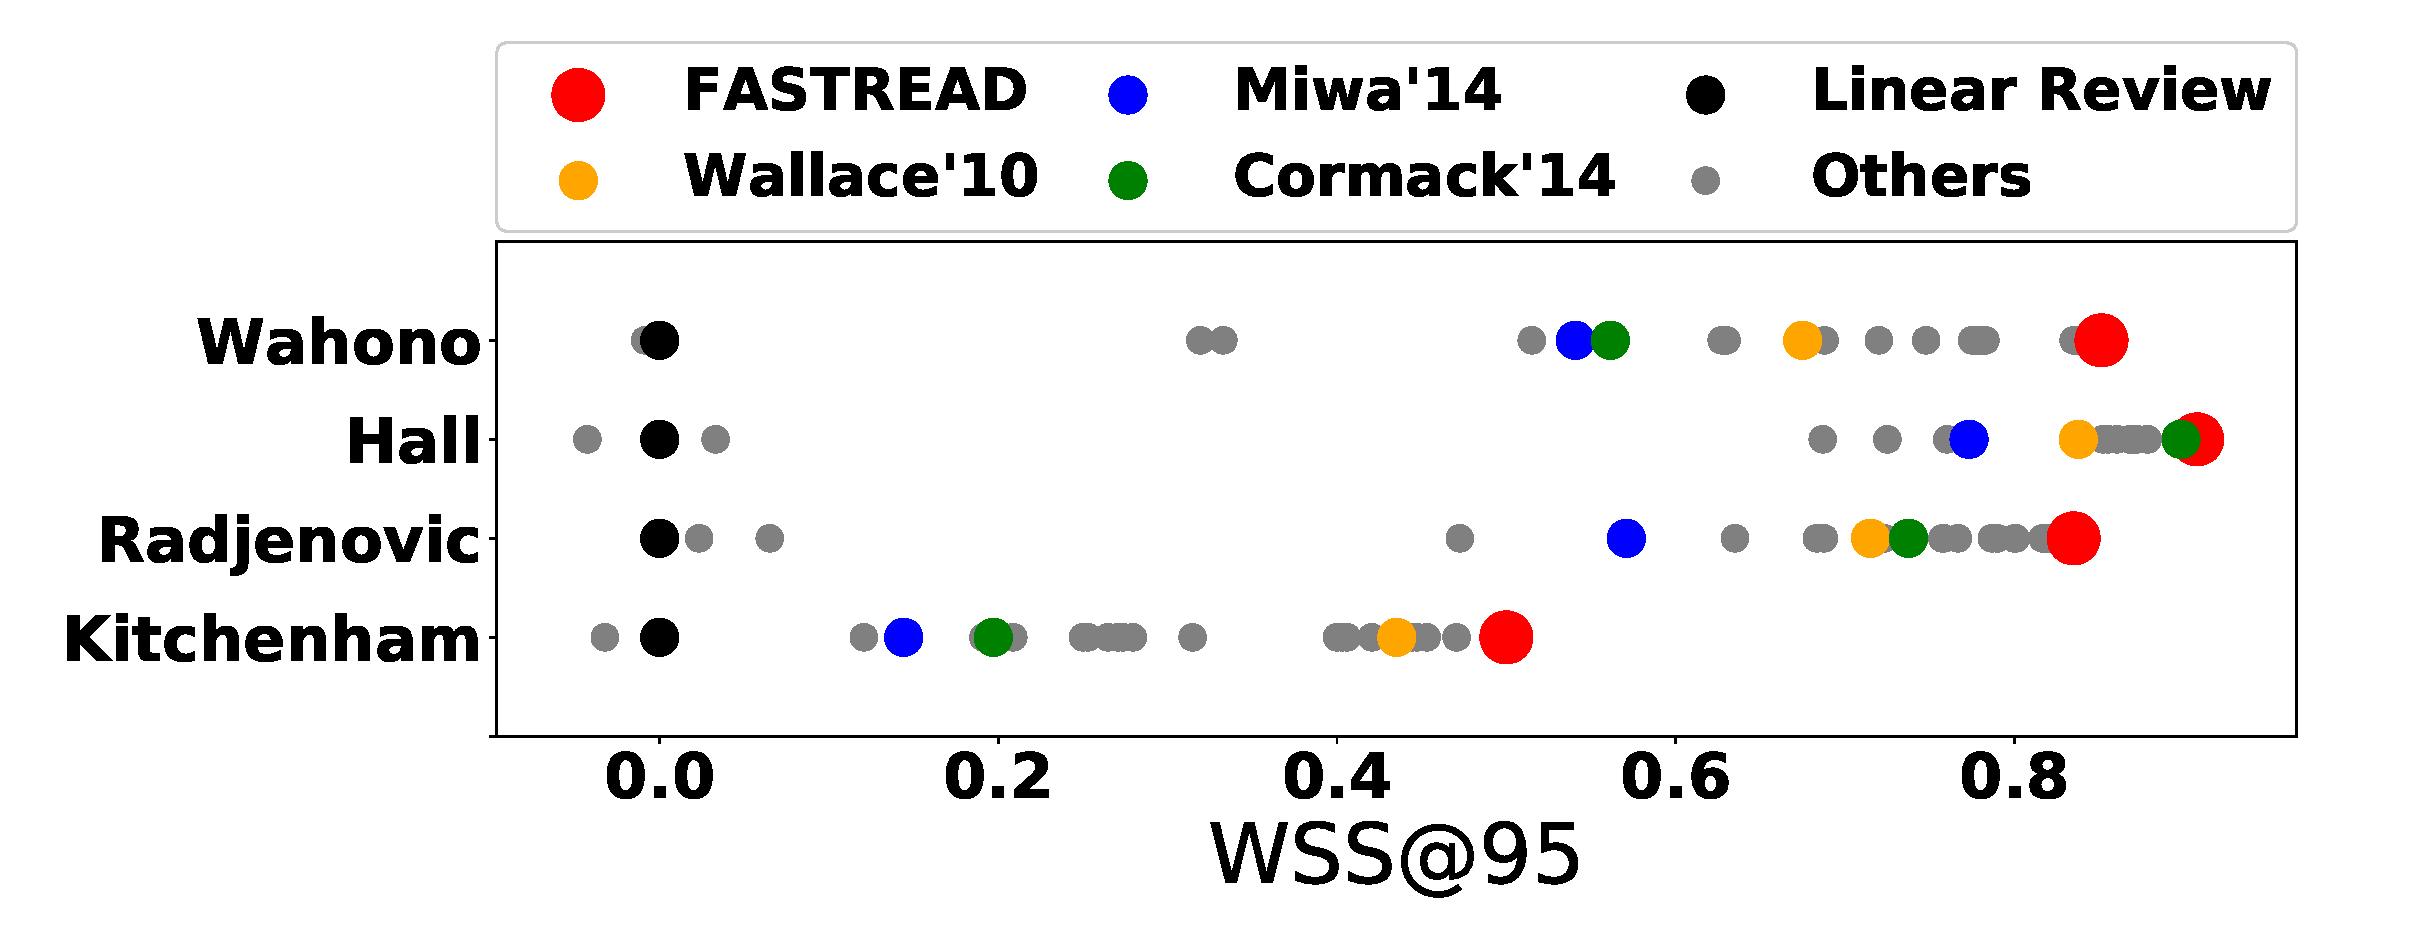
\includegraphics[width=1\linewidth]{figure_codes_chart.eps}
    \caption{FASTREAD (shown in red) performs best compared to  other methods~\cite{cormack2014evaluation,wallace2010active,miwa2014reducing}.
 The x-axis shows  WSS@95:  the number of papers that can be ignored to find 95\% of the relevant papers
    (so {\em larger} WSS@95 values are {\em better}).
Figure shows
median results (over 30 runs) of 32 active learning algorithms and manual review (see ``linear review'') 
using data from   recent prominent SE SLRs: 
    Hall~\cite{hall2012systematic}, Wahono~\cite{wahono2015systematic}, Radjenovi{\'c}~\cite{radjenovic2013software}, Kitchenham et al.~\cite{kitchenham2013systematic}.
    }
    \label{fig:Core}
\end{wrapfigure} 

We do not mean to suggest that {\IT} will {\em only} consist of FASTREAD. {\IT} will comprise many other methods including:
\bii
\item
Topic models, generated from LDA tools~\cite{Biggers-etal:12},  are an excellent way to report and view  textual clusters.
\item
Consider the support vectors of \fig{svm}. FASTEAD used these for the ``select relevant papers'' step of \tbl{overview}.
But the same vectors might also be used to audit any search string proposed in   ``create search string'' (e.g. if search strings do not distinguish the support vectors, then   adjust them).
\item
Given the relatively small size of the SE corpus, AI tools could
cluster that corpus then preemptively run certain queries in anticipation
of possible future queries.
\item
Many more applications of AI-based text mining tools are discussed in \tbl{overview}.
\eii
Our point here is that  AI methods   could be used in so many ways that, as a community, SE researchers need to come together to debate what is useful/required or pointless/depreciated.   The aim of this proposal is to provide the {\IT} infrastructure within which that debate can happen. 

(Note also that as a side-effect of that debate,
{\IT} will also support  practitioners and  researchers to complete their literature reviews better and faster.)
\vspace{8pt}

\subsection{Can AI Address the Requirements of am SLR Tool?}\label{tion:canai}
\noindent

\tion{results} listed several requirements for a useful SLR tool. This section discusses how well
AI-enhanced SLRs can address
those requirements.
Before reviewing those requirements, we digress to make two general points about  AI-enhanced tools like FASTREAD:
\bi
\item
In the sampling processing described above, an active learner (a)~looks for informative examples, then (b)~asks humans comment on those examples. That is, an active learner  routinely  consult with  human beings. This makes such AI-enhanced tools a natural method for combining the automatic and manual methods of \tbl{overview}. For example, when the AI asks the human for an
opinion, the humans could pause the program while they consider what best to say to the AI. During that pause, humans would be free
to gather any additional information they like, perhaps by conducting one of more manual steps within \tbl{overview}.
\item
With active learners,  it is simple to implement a ``reset-and-replay'' policy.
The significance of this is discussed below. But for now, we describe ``reset-and-replay'' as
follows.
The main loop of an active learner builds models $M_1, M_2, M_3,...$ in response to user
feedback obtained after seeing data $D1, D2, D3,...$.
At anytime, a human can return to some prior data point $D_i$, revise their feedback 
after which time and the system can
quickly make models $M'_{j>i}$ by running  through $D_{j>i}$. During that replay step, the user need only be asked
questions 
if model $M'_j$ disagrees with the  old model $M_j$ about data item $D_j$. In our experience, once we have processed more than a small
chunk of the possible examples (say, 10\%), this approach leads to just a handful of disagreements~\cite{Yu20}. That is to say, reset-and-replay is not necessarily an onerous  process for a human being.
\ei
Turning now to the requirements of \tion{results}:

{\em 1. Support task automation -- substitute algorithmic and computer cycles for human work}. We saw above that AI-enhanced SLR tools can augment analysis human of documents.

\begin{wrapfigure}{r}{4in}
\begin{center}
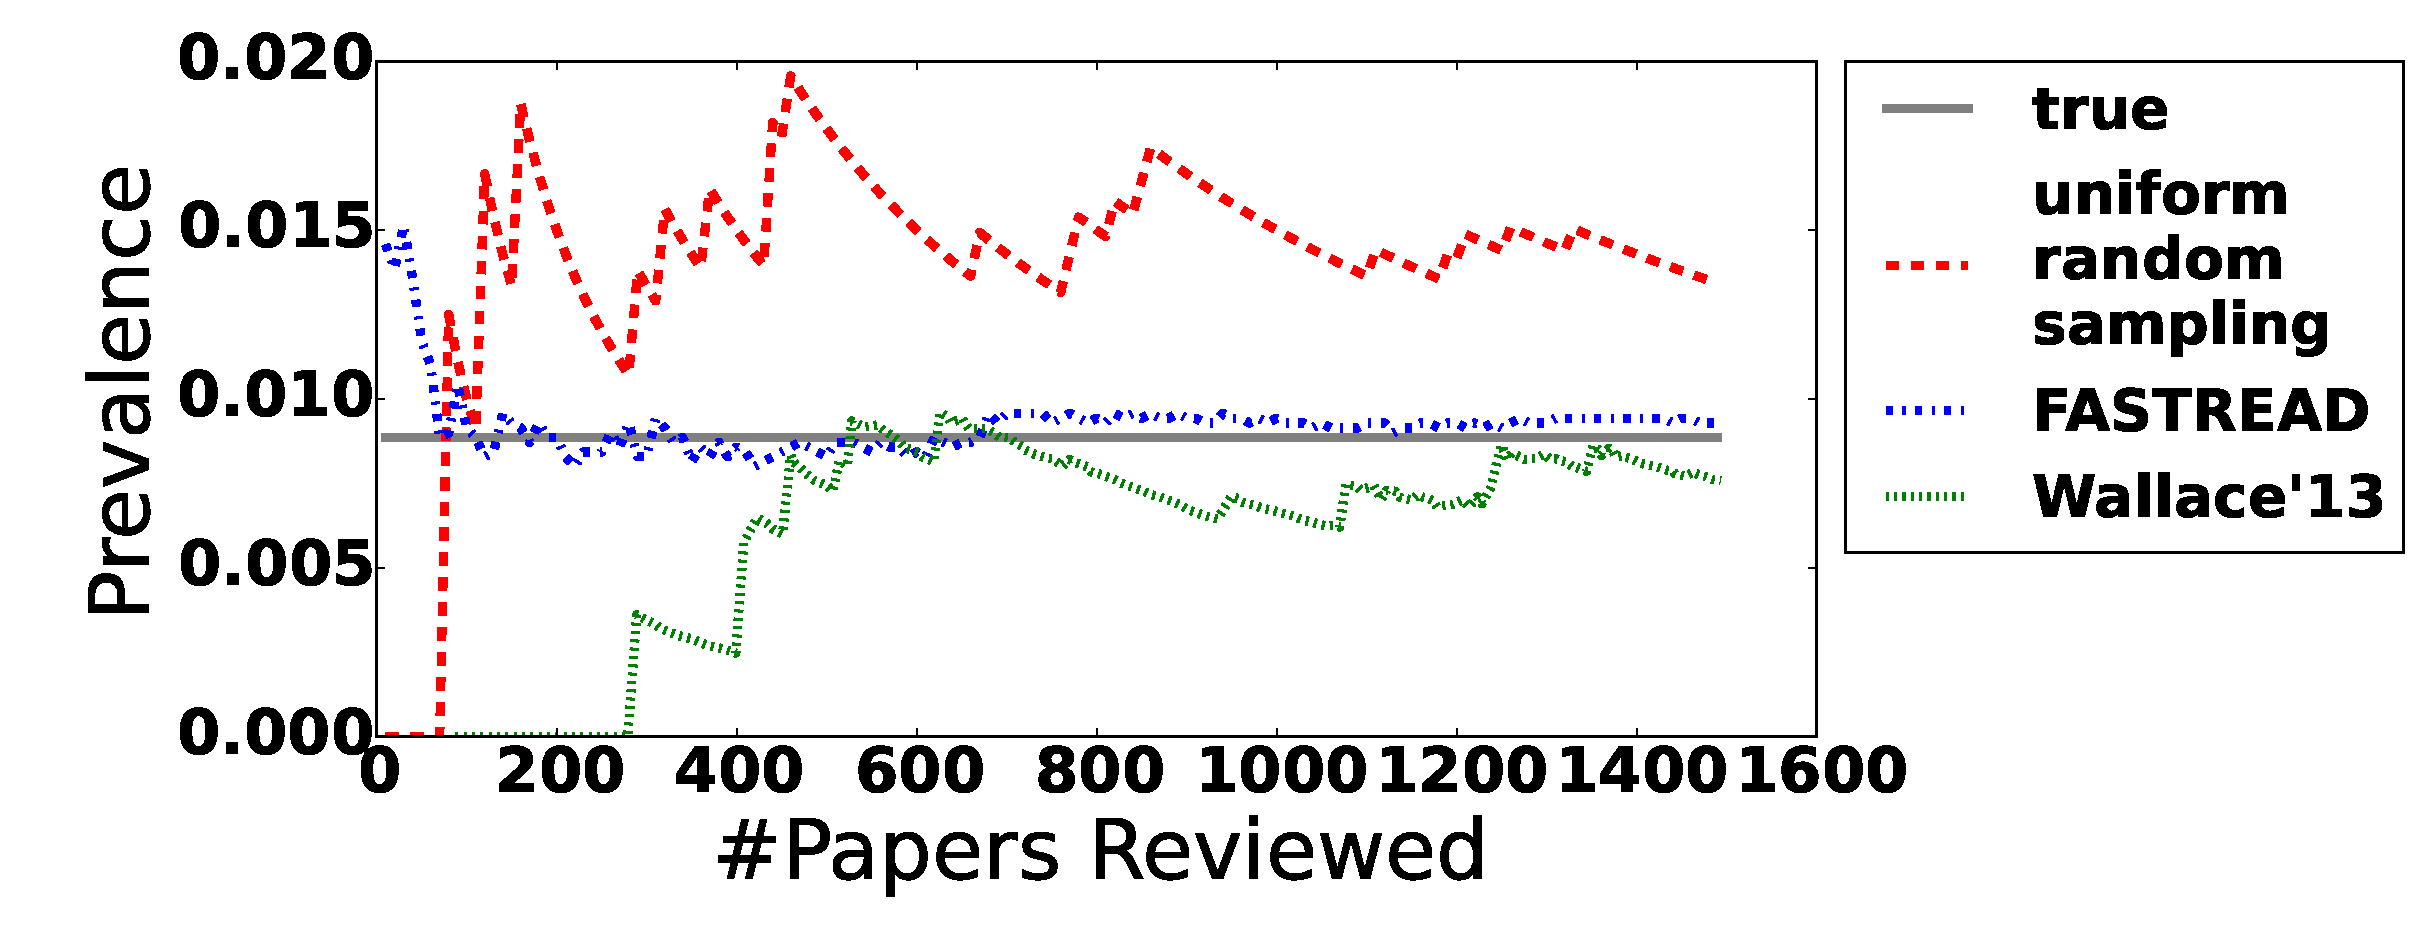
\includegraphics[width=4in]{figure_prev_all_Wahono.eps}
\end{center}
\caption{Guessing how many relevant documents are left to find.
The horizontal gray line denotes perfect predictions. The blue line denotes
results from the FASTREAD predictor for how many papers are left to read.
The red and green line show results from two other methods from the literature~\cite{wallace2013active}. As can be see, with FASTREAD, we quickly learn a
model that can better predict how many relevant documents are left to find.
}\label{fig:error}
\end{wrapfigure}	
~{\em 2. Support automated guidance}. AI-enhanced tools  reflect over their internal models to offer commentary on the progress so far within an SLR.
		For example,  FASTREAD includes tools for predicting how
many relevant documents will be found, after this point. It turns out, with semi-supervised learning, it is possible to accurately predict how many more documents are there to be found during the active learning process.  Using this predictor,
humans can decide for themselves if the 
extra reading effort is worth the reward
of finding more paper. 
There are many ways to build such a predictor but as shown by FASTREAD's \textcolor{blue}{{\bf BLUE}} curve in
\fig{error}, the predictor seen in FASTREAD performs much better than others. In fact, in the case study of \fig{error}, the \textcolor{blue}{{\bf BLUE}} curve's predictions became very close to the actual values very early (after reviewing less than 100 documents).

This facility (that recognizes if it is valid to stop early), is a prime example of the benefits of our proposed combined human+artificial  intelligence. Humans are busy people who must juggle numerous time commitments. Systems that can tell people when ``enough is enough'' gives humans more options on how to balance their busy schedules.

{\em 3. Support iteration within and among SLR Phases}. An SLR is not
		a linear process. Rather, it is often an experimental process in which an analysts makes numerous repeated passes through some data. To support this, AI-enhanced SLR tools can use ``reset-and-replay`` to backup and then revise some prior decision.  

{\em 4. Support project collaboration and coordination of work teams.}
When teams work together it is very useful to have version control tools.
Such version control lets a team fix bad decisions made earlier in the development.
For SLRs, the equivalent to version control is our ``reset-and-replay'' mechanism.
		That is, ``reset-and-replay'' allows teams to store, replay,  reset, forget, enhance    decisions made by individual team members about the relevance of  specific documents.  

{\em 5. Support monitoring of progress and quality.} 
		We saw before in \fig{error} that AI tools   let us apply rigorous evaluation criteria to literature reviews. And such AI tools can offer other quality control help.
		If humans spend hours reviewing documents then, at some point, they may get tired and make a mistake (e.g. label the wrong document as relevant or otherwise). Using ``reset-and-replay'' , AI-enhanced SLR tools   can detect and fix those mistakes.    To do this, we occasionally take the  latest $n$-th version of the classifier and re-applies to to old examples $1\le i < n$. When those new classifications disagree with the old ones, we
		asks humans to review their old labels. In this way, with minimal further samples, AI-enhanced
		SLR tools can alert humans to problems in their labels and tell them exactly where to fix the problem (for more details on this process, see our  paper~\cite{Yu2019}). 

{\em 6.  Support revised planning}; i.e. allow an analyst to update and old literature review. We discussed above that, since the total space of SE papers is not especially larger,  
  it should be possible to pre-compute and cache certain queries, thus reducing the time required to process future queries (as proposed by the {\em Dcluster, Qcluster} methods proposed in row ``1a. Define research question''   of \tbl{overview}).


{\em 7. Support data interchange across all SLR phases.} In principle, {\IT} will enable data interchange between all the methods of \tbl{overview}. That said, we anticipate that
		the design of an appropriate data interchange format between all these methods will
		take considerable time within this project. That said, we have implemented this kind
		of interchange format between multiple AI tools before~\cite{xia19}. Hence we can assert
		that while this work takes time, it is hardly an insurmountable task.

{\em 8. Support existing and future tools through workflow integration and data interchange.} Based on our work building ``glue'' to build interfaces between different AI tools~\cite{gay11,xia19}, we offer a ``rule of 12''; i.e. by the time we have debugged the interface between a dozen  small tools,  then interfacing more tools becomes progressively easier. Hence we anticipate that once we ``glue'' together the methods of \tbl{overview}, we will be situated to combine many more tools in the future.
		
{\em 9. Support an open architecture.} As mentioned above, {\IT} will be an open
		source architecture, freely available on Gitbub. This architecture will be used by several graduate students all trying to publish papers in order to earn their Ph.Ds.
		Further, this architecture will be frequently reviewed by outsiders over the course of this project (at the workshops that we will organize as part of this work). Based on that, we can anticipate many papers describing how to use and improve our open source tools.

\ei
\vspace{8pt}
\newpage
 
